\documentclass[12pt,a4paper]{article}
\usepackage[utf8]{inputenc}
\usepackage{geometry}
\usepackage{graphicx}
\usepackage{amsmath}
\usepackage{hyperref}
\usepackage{fancyhdr}
\usepackage{float}
\usepackage{longtable}
\usepackage{booktabs} 
\usepackage{array}   
\usepackage{enumitem}

% Page layout
\geometry{top=1in, bottom=1in, left=1in, right=1in}

% Title settings
\title{
    \begin{center}
        \textbf{\Huge Deep Learning Course \\ Final Project Report} \\
        \vspace{1cm}
        
\includegraphics[width=0.3\textwidth]{images/logo_unhas.png} \\ 
        \vspace{1cm}
        \textbf{\Large Sistem Informasi Cerdas} 
        \vspace{2cm} 
    \end{center}
}
\author{Rasyad Bimasatya (H071221024)\\ Minhajul Yusri Khairi (H071221006) \\ Andi Ahmad Fa'il Fudhayl (H071221026)}

\date{
    \begin{center}
        \vspace{5cm}
        \textbf{Universitas Hasanuddin} \\
        Makassar, Indonesia \\
        \today
    \end{center}
}

\begin{document}

% Title page
\maketitle

% New page for Table of Contents
\newpage
\tableofcontents
\newpage

% 1. Introduction
\section{Pendahuluan}

Pada era modern, lahir kesadaran negara-negara yang bernuansa Islam untuk membentuk suatu wadah atau forum ulama yang terorganisir dan sistemik untuk mewadahi para mufti dalam lembaga resmi. Di Indonesia, wadah ini dikenal sebagai Majelis Ulama Indonesia (MUI) yang berdiri sejak 1975 berwenang mengeluarkan fatwa di bidang keagamaan, secara khusus di bidang hukum Islam. Kedudukan fatwa dalam konstruksi hukum Islam dapat dikaji dari pengertian fatwa itu sendiri. Sehingga bila berbicara mengenai fatwa itu sendiri, maka tidak akan lepas dari aspek siapa atau organisasi apa yang membuat fatwa tersebut. Fatwa dikeluarkan oleh para ulama atau ahli fikih Islam yang mampu mengangkat permasalahan akibat kebutuhan siapa yang butuh dasar jawaban sebagai landasan hukum suatu perbuatan atau kegiatan yang sifatnya bisa keagamaan atau nonkeagamaan. 

Fatwa yang dikeluarkan oleh lembaga agama memiliki peran penting dalam mengarahkan praktik keagamaan dan menjawab isu-isu yang muncul dalam masyarakat. Namun, biasanya terdapat ketidaksesuaian antara fatwa yang dikeluarkan dan ajaran yang terkandung dalam Al-Quran dan Al-Hadist. Ketidaksesuaian ini dapat mengakibatkan kebingungan dan ketidakpastian bagi umat dalam menjalankan kehidupan beragama. Menguji keselarasan fatwa dengan teks-teks agama yang ada merupakan tugas yang kompleks dan biasanya dilakukan secara manual oleh para ulama dan cendekiawan. Oleh karena itu, perlu adanya suatu metode otomatis dan objektif yang dapat membantu mengukur keselarasan antara fatwa yang dikeluarkan dengan berlandaskan Al-Qur’an dan Al-Hadist. 

Dalam konteks ini, penerapan kecerdasan buatan (AI) melalui teknik\textit{ Natural Language Processing} (NLP) dapat memberikan alternatif baru untuk membantu menganalisis dan memverifikasi keselarasan fatwa dengan ajaran Islam yang bersumber dari Al-Quran dan Al-Hadist. Dengan memanfaatkan kemampuan AI dalam memproses dan menganalisis teks secara cepat dan akurat, diharapkan dapat ditemukan keselarasan antara fatwa yang dikeluarkan dan aturan agama berdasarkan Al-Quran dan Al-Hadist. Penggunaan AI diharapkan dapat memberikan kontribusi dalam penafsiran hukum agama, serta mendukung lembaga agama dalam mengeluarkan fatwa yang sesuai dengan ajaran yang terkandung dalam Al-Quran dan Al-Hadist. 


% 2. Related Works
\section{Penilitian Terkakit}

Dalam mengidentifikasi kesenjangan studi yang membahas keselarasan fatwa dengan Al-Qur’an dan Al-Hadist, pendekatan \textit{Systematic Literature Review} (SLR) digunakan untuk meninjau secara sistematis penelitian-penelitian yang relevan. Hasil tinjauan ini menjadi dasar dalam mengembangkan metode yang lebih akurat dan sistematis untuk mengukur keselarasan antara Fatwa, Al-Qur’an, dan Al-Hadist.

\begin{longtable}{|p{2cm}|p{2cm}|p{2cm}|p{2cm}|p{2cm}|p{2.5cm}|p{2.5cm}|}
\hline
\textbf{Title} & \textbf{Problem} & \textbf{Methods} & \textbf{Solution} & \textbf{Results} & \textbf{Future Works} & \textbf{Gap} \\ \hline\hline
\endfirsthead
\multicolumn{7}{c}{\textit{(Continued from previous page)}} \\ \hline
\textbf{Title} & \textbf{Problem} & \textbf{Methods} & \textbf{Solution} & \textbf{Results} & \textbf{Future Works} & \textbf{Gap} \\ \hline
\endhead
\multicolumn{7}{c}{\textit{(Continued on next page)}} \\ \hline
\endfoot
\endlastfoot

OTORITAS FATWA KEAGAMAAN DALAM KONTEKS ERA KECERDASAN BUATAN (AI) & Dampak AI pada praktik keagamaan & Pendekatan normatif dengan riset pustaka & Pendekatan etik Islam dalam pengembangan AI & AI harus mematuhi prinsip Islam untuk kebaikan umat & Pengembangan AI dengan etik berbasis Islam & Konflik sikap dalam dunia Islam mengenai AI. \\ \hline

Islamic Fatwa Request Routing via Hierarchical Multi-label Arabic Text Categorization & Klasifikasi multi-label dalam pengalihan fatwa & Metode HOMER untuk klasifikasi multi-label & Sistem klasifikasi untuk mengarahkan permintaan fatwa ke mufti yang relevan & HOMER lebih efektif dibanding binary relevance & Pengujian dengan data lebih besar dan penilaian berbasis mufti & Integrasi sistem berbasis ahli untuk konteks yang lebih holistik. \\ \hline

ISLAM IN THE MIDDLE OF AI (Artificial Intelligence) STRUGGLE: BETWEEN OPPORTUNITIES AND THREATS & Peluang dan ancaman AI dalam Islam & Pendekatan kualitatif dengan analisis literatur & Identifikasi peluang dan ancaman AI dalam konteks Islam & AI dapat membawa manfaat, namun ada kekhawatiran etika & Pengembangan kerangka etika AI berbasis Islam & Kurangnya kerangka etika komprehensif dalam dunia Islam. \\ \hline

Processing the Text of the Holy Quran: a Text Mining Study & Pemrosesan teks Al-Qur'an menggunakan text mining & Teknik TF dan TF-IDF untuk analisis teks & Visualisasi kata-kata penting dalam Al-Qur'an & Hasilkan kata-kata paling sering muncul dalam Al-Qur'an & Pengembangan algoritma stemming bahasa Arab yang lebih akurat & Keterbatasan alat stemming menyebabkan analisis kurang presisi. \\ \hline

\end{longtable}

\begin{figure}[h!]
    \centering
    \caption{Systematic Literature Review}
    \label{fig:slr}
\end{figure}

\newpage
 Penelitian pertama membahas pentingnya kerangka etika dalam penggunaan AI untuk menganalisis fatwa, terutama dalam konteks Islam. Studi ini menekankan perlunya menjaga keseimbangan antara nilai-nilai keagamaan dan kebermanfaatan teknologi. Namun, ditemukan adanya kesenjangan dalam penerapan AI yang dapat memengaruhi praktik keagamaan akibat konflik antara dampak positif dan negatifnya \cite{Hakim2023}.

 Selanjutnya, penelitian kedua mengusulkan pendekatan \textit{multi-label classification }untuk mengelompokkan dan memproses permintaan fatwa yang kompleks. Pendekatan ini menggunakan metode \textit{Hierarchical Ensembles} untuk meningkatkan akurasi dalam mengelompokkan fatwa sesuai relevansi kategori. Studi ini berhasil meningkatkan efisiensi pengelompokan fatwa, meskipun tantangan tetap ada, terutama dalam mempertimbangkan konteks holistik dari teks keagamaan \cite{Zayed2015}.

 Penelitian ketiga mengeksplorasi peluang dan ancaman penerapan AI dalam memahami nilai-nilai Islam. Peneliti menyoroti bagaimana AI dapat membantu identifikasi nilai-nilai keagamaan, namun mencatat perlunya pembingkaian ulang kerangka kerja etika untuk memastikan penerapannya tidak bertentangan dengan nilai-nilai Islam. Studi ini memberikan wawasan penting tentang tantangan penerapan AI di masyarakat Muslim \cite{Rohman2023}.

 Studi terakhir berfokus pada analisis teks Al-Qur'an menggunakan teknik \textit{text mining }seperti \textit{term frequency-inverse document frequency} (TF-IDF) untuk memahami pola kata dalam teks. Meskipun teknik ini memberikan wawasan baru, penelitian ini belum menerapkan metode \textit{stemming} dalam bahasa Arab yang dapat meningkatkan akurasi analisis \cite{Alhawarat2015}.

Meskipun keempat studi ini memberikan kontribusi penting dalam konteks analisis teks keagamaan dan penerapan AI, hingga saat ini penulis belum menemukan penelitian yang mengaplikasikan NLP untuk memverifikasi kesesuaian fatwa dengan ajaran Al-Quran dan Hadist, khususnya di Indonesia.  Sehingga ini diharapkan menjadi pionir dalam penerapan NLP untuk analisis hukum Islam dan dapat membuka peluang bagi studi lebih lanjut dalam verifikasi kesesuaian fatwa di dunia akademik maupun praktik keagamaan, serta mempermudah masyarakat dalam memahami panduan yang sahih.



% 3. Dataset and Material
\section{Dataset dan Material}

Studi ini melibatkan tiga sumber data utama, yaitu teks Al-Quran, koleksi Hadist, dan data Fatwa yang digunakan untuk menganalisis keselarasan fatwa dengan ajaran Islam yang terkandung dalam Al-Quran dan Hadist. Penjelasan berikut menguraikan lebih lanjut mengenai sumber data yang digunakan, teknik pengumpulan data, serta langkah-langkah \textit{pre-processing} yang diterapkan.

\subsection{Sumber Data}

\begin{itemize}
    \item \textbf{Data Al-Quran:} 
    Data Al-Quran yang digunakan diperoleh dari situs web resmi \href{http://quran.nu.or.id/}{quran.nu.or.id}. Al-Quran yang digunakan mencakup 114 surah dengan total 6236 ayat. Pengambilan data dilakukan menggunakan teknik \textit{web scraping} dengan menggunakan Selenium WebDriver dan lxml. Selenium WebDriver dipilih untuk mengotomatisasi proses pengambilan data secara dinamis dari situs web, sementara lxml digunakan untuk memproses dan mengekstrak elemen-elemen teks dari halaman web yang berisi teks Al-Quran.

    \begin{figure}[h!]
        \centering
        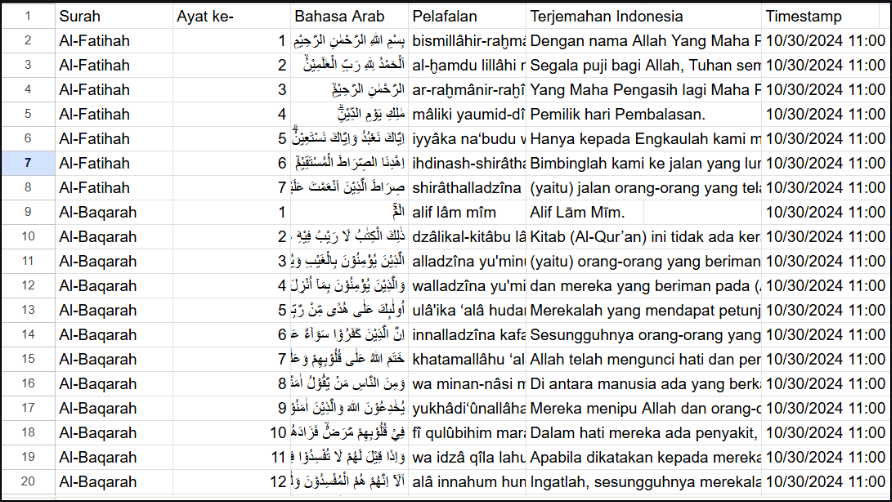
\includegraphics[width=0.8\textwidth]{images/quran.png}
        \caption{Data Al-Qur'an}
        \label{fig:quran}
    \end{figure}

    \item \textbf{Data Hadist:} 
    Data Hadist yang digunakan dalam studi ini diambil dari \href{https://ilmuislam.id/hadits/perawi/2/ahmad}{ilmuislam.id}, sebuah situs yang menyediakan berbagai riwayat hadist yang dapat diakses secara terbuka. Total 9 riwayat Hadist yang digunakan dalam penelitian ini meliputi:
    \begin{itemize}
        \item Abu Daud
        \item Ahmad
        \item Buhari
        \item Darimi
        \item Ibnu Majah
        \item Malik
        \item Muslim
        \item Nasai
        \item Tirmidzi
    \end{itemize}
    
    Data Hadist diambil dengan menggunakan teknik \textit{scraping} yang sama seperti yang digunakan untuk Al-Quran, yaitu dengan Selenium WebDriver dan lxml. Teknik ini memastikan bahwa teks Hadist yang diambil dari situs web dapat diproses dengan cepat dan tepat.

    \begin{figure}[h!]
        \centering
        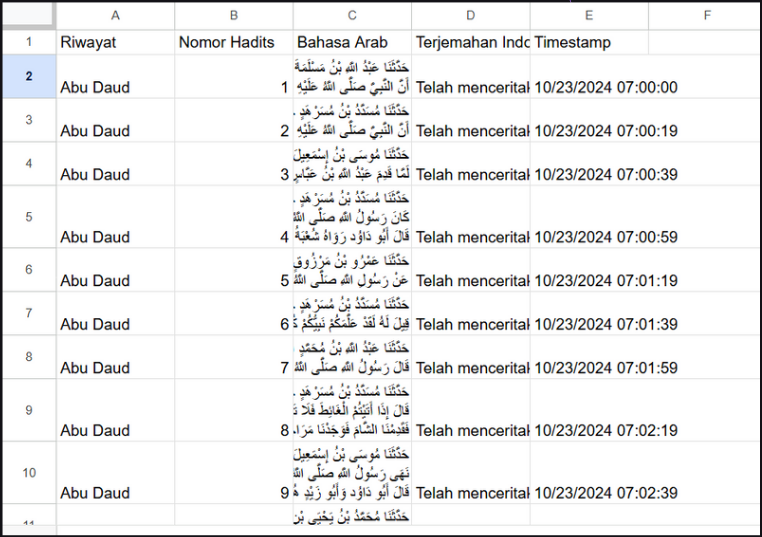
\includegraphics[width=0.8\textwidth]{images/hadist.png}
        \caption{Data Hadist}
        \label{fig:hadist}
    \end{figure}

    \newpage
    \item \textbf{Data Fatwa:} 
    Data fatwa yang digunakan diambil dari \href{https://fatwamui.com/data-fatwa}{fatwamui.com}, sebuah portal resmi yang menyediakan fatwa dari Majelis Ulama Indonesia (MUI). Fatwa yang digunakan berjumlah 344 sample. Data ini dikumpulkan secara manual karena pola untuk mencari bagian fatwa pada file PDF sulit ditemukan, sehingga semua fatwa tidak dapat diakses langsung melalui metode \textit{scraping}. 

    \begin{figure}[h!]
        \centering
        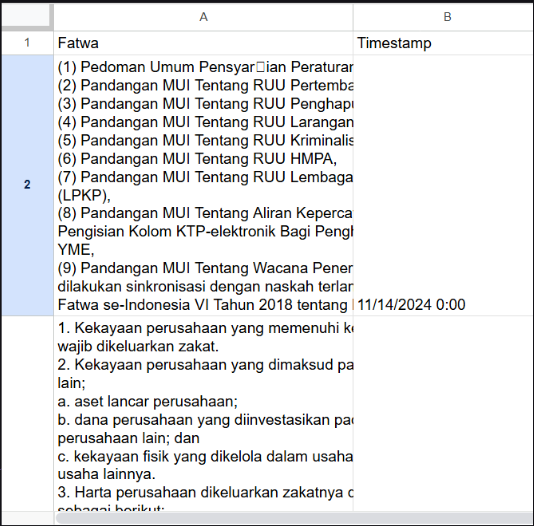
\includegraphics[width=0.8\textwidth, height=10cm]{images/fatwa.png}
        \caption{Data Fatwa}
        \label{fig:fatwa}
    \end{figure}
\end{itemize}

\newpage
\subsection{Data Preprocessing}

Setelah data terkumpul, dilakukan beberapa langkah \textit{pre-processing} untuk mempersiapkan data agar dapat dianalisis lebih lanjut. Langkah-langkah \textit{pre-processing} yang dilakukan adalah sebagai berikut:

\begin{itemize}
    \item \textbf{\textit{Lowercase Text}:} Semua teks yang dikumpulkan, baik dari Al-Quran, Hadist, maupun fatwa, diubah menjadi huruf kecil untuk memastikan konsistensi. Hal ini penting karena dalam analisis teks, perbedaan kapitalisasi antara kata-kata yang serupa dapat menyebabkan inkonsistensi dan kesalahan dalam pencocokan kata.
    
    \item \textbf{\textit{Remove Punctuations and Extra Spaces}:} Tanda baca seperti koma, titik, tanda tanya, dan lainnya dihapus dari teks. Selain itu, spasi tambahan juga dihilangkan untuk memperbaiki kualitas teks dan memastikan analisis yang lebih bersih. Langkah ini bertujuan untuk mengurangi kebisingan dalam teks yang tidak memberikan kontribusi pada analisis makna.

    \item \textbf{\textit{Stopwords Removal}:} \textit{Stopwords} adalah kata-kata yang sering muncul dalam teks tetapi tidak membawa banyak makna atau informasi penting (misalnya, "dan", "yang", "dari"). Kata-kata ini dihapus karena mereka dapat mengganggu proses pencocokan teks. Penghapusan \textit{stopwords} dilakukan dengan menggunakan daftar\textit{ stopwords} bahasa Indonesia yang sudah tersedia dalam pustaka NLP.

    \item \textbf{\textit{Stemming}:}\textit{ Stemming} adalah proses mengubah kata-kata turunan menjadi bentuk dasar atau akar katanya. Misalnya, kata “berdoa” akan diubah menjadi “doa”. Proses ini penting untuk menyatukan kata-kata yang memiliki arti serupa namun ditulis dalam bentuk yang berbeda, sehingga pencocokan teks lebih akurat. Teknik \textit{stemming} ini diterapkan menggunakan pustaka NLP untuk bahasa Indonesia.
\end{itemize}

\subsection{Fitur dan Label}
Fitur yang digunakan untuk melatih model \textit{deep learning} mencakup teks Fatwa, teks Al-Qur'an, dan teks Hadist. Ketiga teks ini terlebih dahulu diproses menggunakan \textit{word embedding}, yang bertujuan mengubah kata-kata menjadi representasi numerik dalam bentuk vektor. Karena tidak tersedia label yang secara langsung mengukur skor keselarasan antara teks, penelitian ini mengadopsi pendekatan \textit{pseudo-labelling} untuk menciptakan label semu secara otomatis.

\textit{Pseudo-labelling} adalah metode \textit{semi-supervised learning} yang memanfaatkan data tidak berlabel dengan cara membuat prediksi awal menggunakan model yang sudah dilatih \cite{Kuligowska}. Prediksi ini kemudian digunakan sebagai label semu untuk melatih model lebih lanjut. Pendekatan ini memungkinkan model memanfaatkan informasi tambahan dari data yang sebelumnya tidak berlabel, sehingga dapat meningkatkan kinerja dan akurasi model.

Dalam penelitian ini, dilakukan penggabungan data antara hasil \textit{embedding} dari teks Fatwa dengan teks Al-Qur'an, serta hasil \textit{embedding} dari teks Fatwa dengan teks Hadist. Hasil penggabungan ini dimasukkan ke dalam sebuah \textit{dataframe} yang menghasilkan total 15.090.592 kombinasi pasangan. Setiap pasangan kemudian dihitung skor keselarasan menggunakan pendekatan \textit{cosine similarity}. Skor ini mengukur tingkat kesamaan antara vektor-vektor yang mewakili teks-teks tersebut setelah melalui proses\textit{ embedding}. \textit{Cosine similarity} menghitung kesamaan dengan menilai sudut antara dua vektor dalam ruang multidimensi \cite{J.Han}. Semakin kecil sudut tersebut, atau semakin besar nilai cosine similarity, semakin tinggi tingkat keselarasan antara teks-teks yang dibandingkan.

\textit{Cosine similarity} didefinisikan sebagai:

\[
\text{CosineSimilarity}(A, B) = \frac{A \cdot B}{\|A\| \|B\|}
\]

\textbf{Keterangan:}
\begin{itemize}
    \setlength{\itemindent}{1em} % Menambahkan indentasi untuk bullet point
    \item \( A \cdot B \) adalah hasil \textit{dot product} antara vektor \( A \) dan \( B \).
    \item \( \|A\| \) dan \( \|B\| \) adalah norma atau panjang dari vektor \( A \) dan \( B \).
    \item Nilai \(\text{CosineSimilarity}\) berkisar antara -1 hingga 1:
    \begin{itemize}
        \setlength{\itemindent}{2em}
        \item Nilai 1 menunjukkan kesamaan sempurna (vektor searah).
        \item Nilai 0 menunjukkan tidak ada kesamaan (vektor tegak lurus).
        \item Nilai -1 menunjukkan ketidaksamaan total (vektor berlawanan arah).
    \end{itemize}
\end{itemize}

Total kombinasi pasangan antara Fatwa dengan Al-Qur'an dan Fatwa dengan Hadist berjumlah sangat besar, yaitu 15.090.592 kombinasi pasangan. Jika peneliti memaksakan untuk melatih model dengan jumlah sebanyak itu, maka waktu yang dibutuhkan untuk melatih model akan sangat lama. Meskipun peneliti menggunakan GPU NVIDIA GeForce RTX 3060, estimasi waktu yang diperlukan tetap sangat lama, bahkan bisa berhari-hari. Untuk mengatasi masalah ini, peneliti memilih untuk hanya menggunakan pasangan data Fatwa dengan Al-Qur'an dan Fatwa dengan Hadist yang memiliki skor \textit{cosine similarity} tertinggi di setiap pasangannya. Dengan cara ini, jumlah data yang digunakan untuk pelatihan dapat diminimalkan. Total jumlah data yang akan digunakan untuk pelatihan adalah sebanyak 688 pasangan, karena jumlah data Fatwa yang ada sebanyak 344.

\begin{figure}[H]
    \centering
    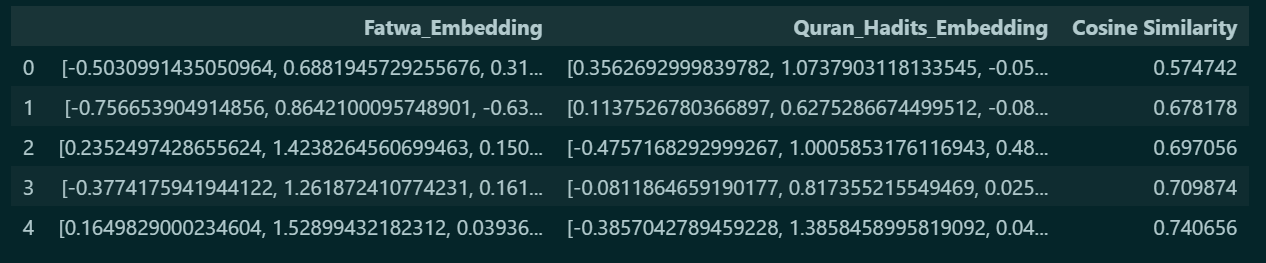
\includegraphics[width=0.9\textwidth]{images/data_embedded.png}
    \caption{Pasangan data yang telah diubah menjadi vektor beserta skor \textit{Cosine Similarity}}
    \label{fig:bert}
\end{figure}

\subsection{Tools dan Libraries}
Beberapa alat utama yang digunakan adalah sebagai berikut:

\begin{itemize}
    \item \textbf{Selenium:} Digunakan untuk melakukan \textit{web scraping} dengan mengotomatisasi interaksi dengan halaman web untuk mengakses dan mengekstrak data teks dari situs Al-Qur'an dan Hadist.
    
    \item \textbf{LXML:} Digunakan untuk memproses HTML dan XML dalam proses \textit{scraping}. lxml memberikan kemampuan untuk memparsing halaman web dan mengekstrak elemen-elemen teks yang diperlukan secara efisien.
    
    \item \textbf{\textit{Natural Language Toolkit} (NLTK):} Pustaka Python yang digunakan untuk pemrosesan bahasa alami, termasuk untuk \textit{stopwords removal} dan \textit{stemming}. NLTK menyediakan berbagai fitur yang berguna untuk \textit{pre-processing} teks dalam bahasa Indonesia.
    
    \item \textbf{Scikit-learn:} Pustaka Python yang digunakan untuk evaluasi dan pengukuran kinerja model, termasuk perhitungan metrik-metrik seperti akurasi dan F1-score, serta pembuatan confusion matrix.

    \item \textbf{NVIDIA GeForce RTX 3060:} Digunakan untuk mempercepat proses pelatihan model \textit{deep learning} dengan menyediakan pemrosesan paralel yang efisien menggunakan GPU.
    
    \item \textbf{Visual Studio Code:} Editor kode sumber yang digunakan untuk mengembangkan dan mengedit kode program. Visual Studio Code menyediakan berbagai ekstensi yang mendukung pengembangan dalam bahasa Python.
    
    \item \textbf{TensorFlow:} Pustaka open-source untuk \textit{machine learning} dan \textit{deep learning}, yang digunakan untuk membangun dan melatih model-model pembelajaran mendalam dalam penelitian ini.
    
    \item \textbf{PyTorch:} Pustaka open-source lain untuk \textit{deep learning}, yang digunakan dalam pengembangan dan pelatihan model \textit{neural network} dalam penelitian ini.

    \item \textbf{Sastrawi:} Pustaka Python untuk \textit{stemmer} bahasa Indonesia yang digunakan dalam proses \textit{pre-processing} teks untuk mengurangi kata-kata menjadi bentuk dasarnya.

    \item \textbf{Matplotlib:} Pustaka Python yang digunakan untuk menghasilkan visualisasi grafis, seperti grafik dan diagram, yang membantu dalam menganalisis dan memvisualisasikan hasil eksperimen.
    
    \item \textbf{Seaborn:} Pustaka visualisasi data berbasis Matplotlib yang digunakan untuk membuat plot statistik yang lebih menarik dan informatif.
\end{itemize}


\subsection{Model}
Model yang dipakai untuk menguji keselarasan antara  fatwa yang dikeluarkan dengan Al-Qur’an dan Al-Hadist adalah IndoBERT dan \textit{Long Short-Term Memory} (LSTM). Berikut ini penjelasannya:

\begin{itemize}
    \item \textbf{IndoBERT:} IndoBERT adalah salah satu model terbaik untuk analisis teks dalam bahasa Indonesia. Arsitektur IndoBERT dibangun menggunakan model \textit{transformer} seperti BERT pada umumnya, yang awalnya dirancang untuk bahasa Inggris. IndoBERT menggunakan 12 \textit{hidden layers}, dengan masing-masing lapisan memiliki dimensi 786, serta 12 \textit{attention heads} \cite{Juarto2023}. Model ini dilatih menggunakan lebih dari 220 juta kata dalam bahasa Indonesia yang diambil dari sumber-sumber yang menggunakan bahasa Indonesia yang baik dan benar, seperti koran online, Indonesian Web Corpus, dan sumber-sumber lainnya.

    \begin{figure}[H]
        \centering
        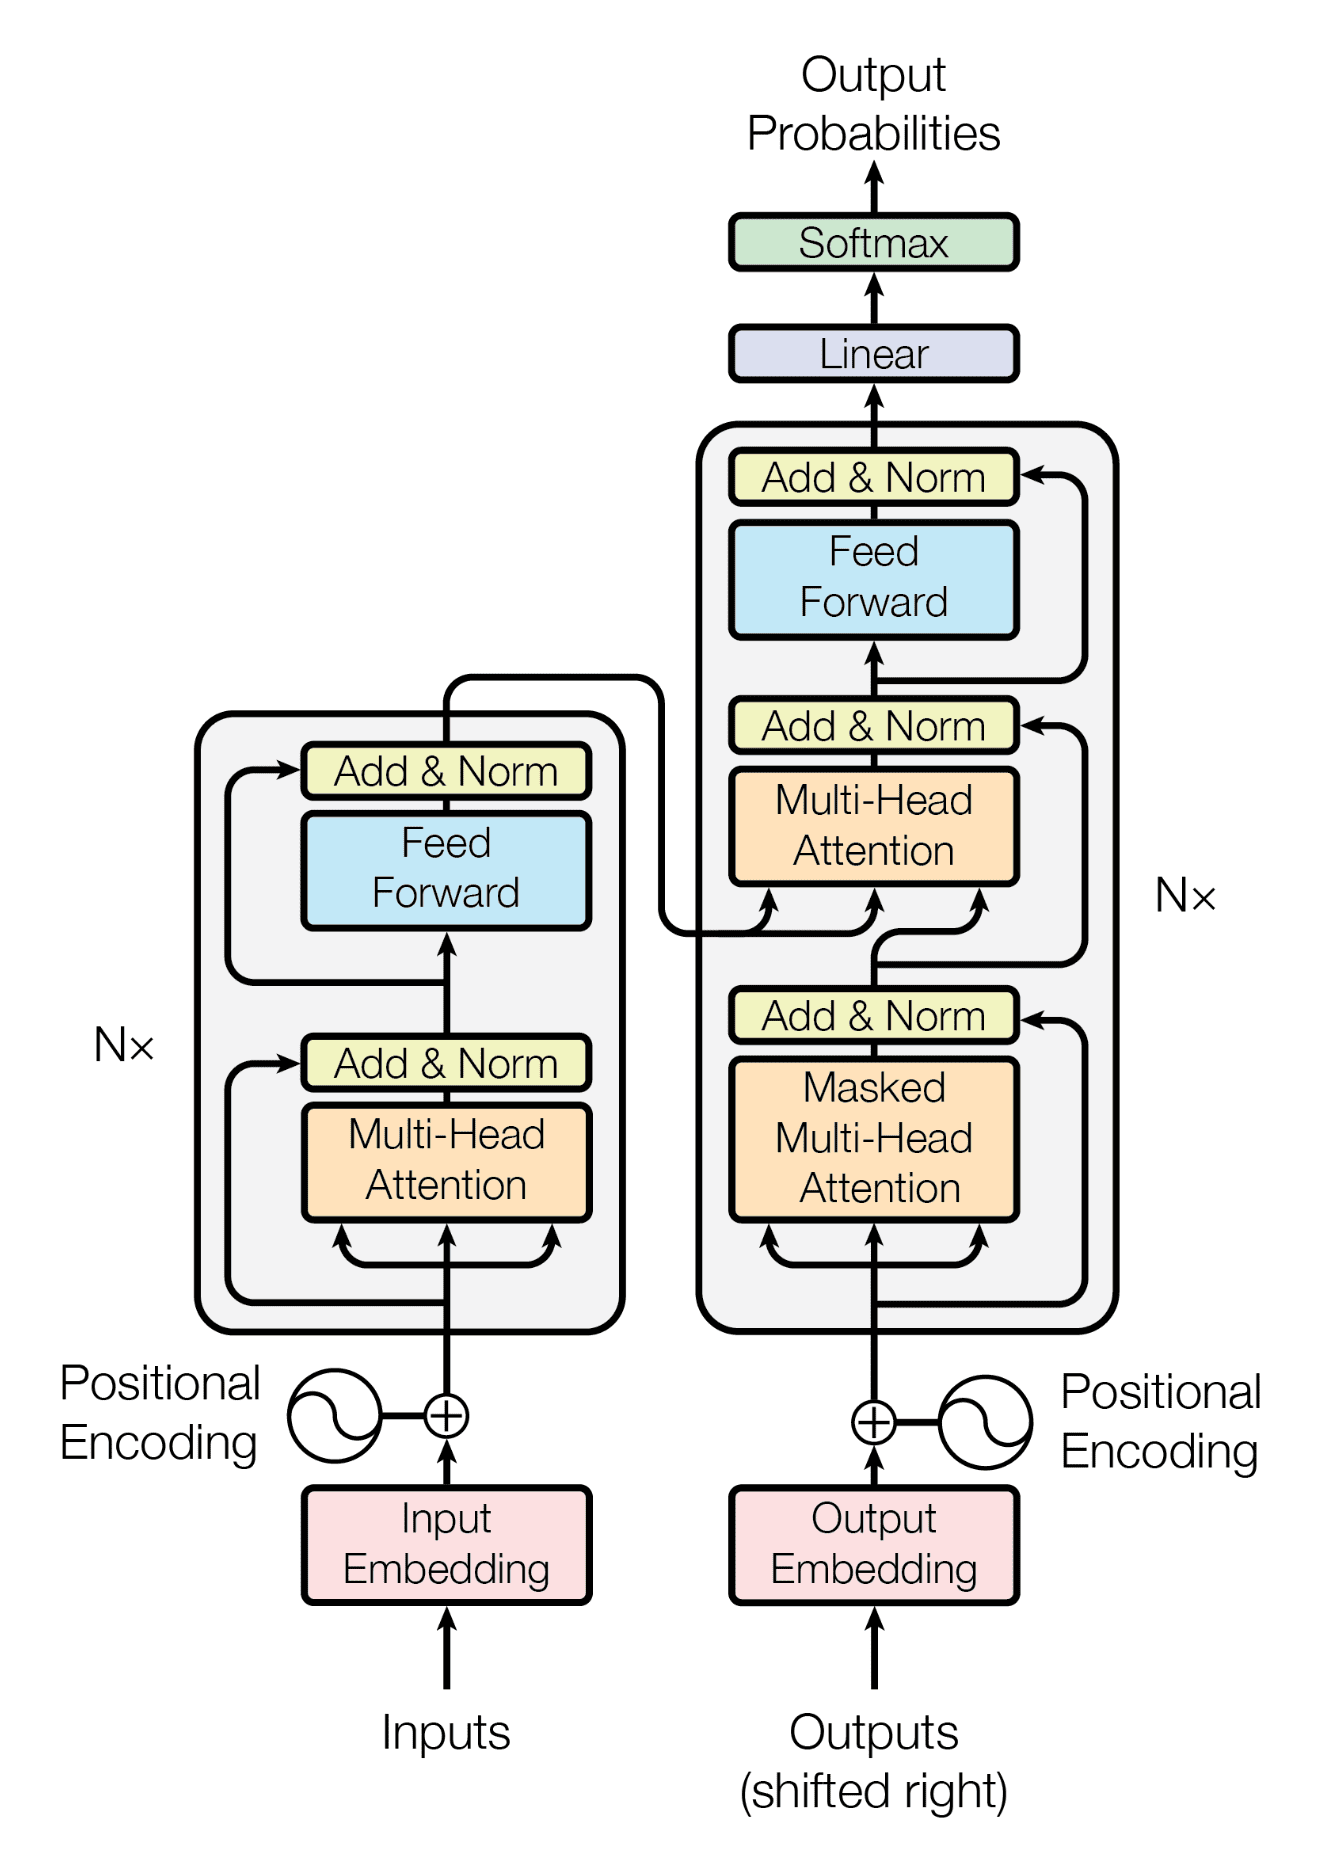
\includegraphics[width=0.5\textwidth]{images/bert.png}
        \caption{Arsitektur IndoBERT}
        \label{fig:bert}
    \end{figure}

    BERT memiliki \textit{encoder} dan \textit{decoder} dalam arsitekturnya. Perbedaannya terletak pada \textit{encoder} yang fungsinya untuk menerima input dan mengubahnya menjadi vektor kata, sementara \textit{decoder} berfungsi untuk membuat prediksi dari berbagai tugas. Agar kata-kata dapat diubah menjadi vektor di dalam \textit{encoder}, BERT memiliki tiga jenis \textit{embedding}. Hal ini karena model BERT membuat model bahasa yang dapat direpresentasikan dengan baik dalam bentuk vektor sehingga dapat memberikan hasil model prediksi yang baik. Beberapa \textit{embedding} yang diterapkan dalam input BERT antara lain:
    \begin{itemize}
        \item \textbf{\textit{Token embedding}s:} Token-token yang berada di awal kalimat direpresentasikan dengan \texttt{[CLS]}, sementara di akhir kalimat direpresentasikan dengan token \texttt{[SEP]}.
        \item \textbf{\textit{Embeddings segment}:} \textit{Embedding }ini berguna untuk membedakan antara dua kalimat dengan menandai setiap kalimat.
        \item \textbf{\textit{Positional embeddings}:} \textit{Embedding }ini memberikan token yang berguna untuk menyediakan informasi posisi pada embedding dalam sebuah kalimat.
    \end{itemize}

    \begin{figure}[H]
        \centering
        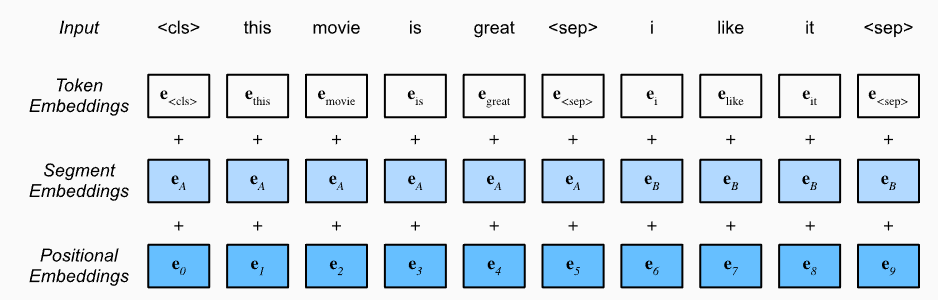
\includegraphics[width=0.8\textwidth]{images/embedding.png}
        \caption{3 Jenis Embedding BERT}
        \label{fig:embedding}
    \end{figure}

    Dalam penelitian ini, IndoBERT digunakan untuk mengubah teks Fatwa, Al-Qur'an, dan Hadist menjadi representasi vektor melalui proses \textit{word embedding}. Setiap pasangan Fatwa dengan Al-Qur'an atau Fatwa dengan Hadist kemudian dihitung skor keselarasan menggunakan \textit{cosine similarity} pada hasil \textit{embedding} tersebut. Selanjutnya, IndoBERT juga digunakan dalam tahap \textit{fine-tuning} untuk melatih model yang lebih spesifik pada domain Fatwa, Al-Qur'an, dan Hadist.

    \item \textbf{\textit{Long Short-Term Memory} (LSTM):} LSTM adalah jenis jaringan saraf tiruan yang digunakan untuk mengatasi masalah yang ada pada jaringan saraf biasa, yaitu masalah pembelajaran jangka panjang. LSTM dikembangkan untuk mengatasi kesulitan dalam melatih jaringan saraf berlapis banyak, khususnya dalam memproses urutan data yang panjang, seperti teks dan waktu. Jaringan LSTM diperkenalkan oleh Hochreiter dan Schmidhuber pada tahun 1997 dan menjadi populer karena kemampuannya untuk menangani informasi dalam jangka panjang \cite{hochreiter1997long}.

    Arsitektur LSTM adalah bentuk khusus dari jaringan \textit{Recurrent Neural Networks} (RNNs) yang menggunakan unit memori untuk memproses informasi secara berurutan. Berbeda dengan RNN biasa, LSTM memiliki kemampuan untuk memutuskan kapan harus menyimpan, membaca, dan menghapus informasi dari memori. Ini memungkinkan LSTM untuk mengingat informasi penting dari langkah-langkah sebelumnya dalam urutan input untuk waktu yang lebih lama \cite{Graves}. LSTM memiliki tiga gerbang utama yang mengatur aliran informasi \cite{hochreiter1997long}:
    \begin{itemize}
        \item \textbf{Forget Gate:} Gerbang ini memutuskan informasi mana yang harus dilupakan dari unit memori. Ini berdasarkan input saat ini dan status sebelumnya.
        \item \textbf{Input Gate:} Gerbang ini mengontrol informasi baru yang akan disimpan dalam unit memori. Gerbang ini memutuskan seberapa besar bagian dari informasi yang akan disimpan berdasarkan input saat ini dan status sebelumnya.
        \item \textbf{Output Gate:} Gerbang ini memutuskan output dari unit LSTM berdasarkan memori yang ada. Output yang dihasilkan akan digunakan untuk langkah berikutnya dalam urutan atau sebagai hasil prediksi akhir.
    \end{itemize}

    \begin{figure}[H]
        \centering
        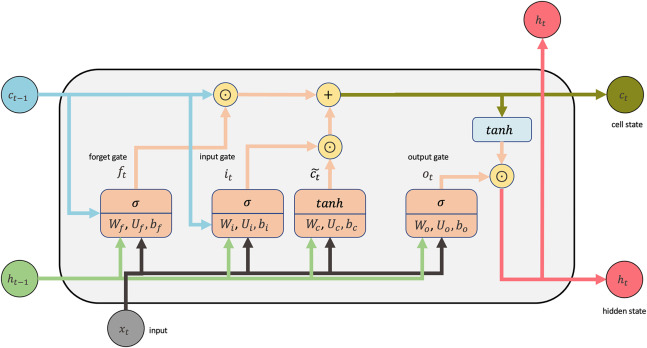
\includegraphics[width=0.8\textwidth]{images/lstm.jpg}
        \caption{Arsitektur \textit{Long Short-Term Memory} (LSTM)}
        \label{fig:lstm}
    \end{figure}

    Dalam penelitian ini, LSTM digunakan untuk mempelajari hubungan temporal antara teks Fatwa, Al-Qur'an, dan Hadis. LSTM dapat mengingat konteks dan memproses urutan kata-kata yang lebih panjang, yang membantu model dalam menentukan sejauh mana keselarasan antara Fatwa dengan Al-Quran dan Hadist.

\end{itemize}

\subsection{Optimizer}

Pada kedua model yang digunakan dalam penelitian ini, yaitu model berbasis IndoBERT dan \textit{Long Short-Term Memory} (LSTM), digunakan optimasi \textit{Adaptive Moment Estimation} (ADAM) selama proses pelatihan model.

\begin{itemize}
    \item \textbf{\textit{Adaptive Moment Estimation} (ADAM)}: Adam adalah metode adaptif yang menggabungkan kelebihan dua metode optimasi lainnya, yaitu AdaGrad dan RMSProp. Adam memperbarui parameter model dengan menghitung estimasi rata-rata momentum pertama dan momentum kedua. Pendekatan ini memungkinkan Adam untuk secara adaptif menyesuaikan laju pembelajaran untuk setiap parameter secara individual. Hal ini membantu mengatasi masalah seperti gradien yang sangat kecil atau sangat besar, sehingga meningkatkan stabilitas, efisiensi, dan kecepatan konvergensi dibandingkan metode optimasi lainnya \cite{Kingma}.
    
    Adam mengupdate parameter $\theta_t$ pada waktu $t$ menggunakan rumus berikut:
    
    \[
    m_t = \beta_1 m_{t-1} + (1 - \beta_1) g_t
    \]
    \[
    v_t = \beta_2 v_{t-1} + (1 - \beta_2) g_t^2
    \]
    \[
    \hat{m}_t = \frac{m_t}{1 - \beta_1^t}, \quad \hat{v}_t = \frac{v_t}{1 - \beta_2^t}
    \]
    \[
    \theta_t = \theta_{t-1} - \frac{\alpha}{\sqrt{\hat{v}_t} + \epsilon} \hat{m}_t
    \]
    
    Di mana:
    \begin{itemize}
        \item $m_t$ dan $v_t$ adalah estimasi rata-rata pertama dan kedua dari gradien.
        \item $\beta_1$ dan $\beta_2$ adalah parameter momentum yang biasanya diset ke 0.9 dan 0.999.
        \item $g_t$ adalah gradien pada waktu $t$.
        \item $\alpha$ adalah \textit{learning rate} yang mengontrol ukuran langkah pembaruan parameter.
        \item $\epsilon$ adalah konstanta kecil yang digunakan untuk menghindari pembagian dengan nol.
    \end{itemize}
\end{itemize}

% 4. Result and Discussion
\section{Hasil dan Diskusi}
\subsection{Metrik Evaluasi}

Dalam penelitian ini, digunakan beberapa metrik evaluasi untuk mengukur performa model, yaitu\textit{ Mean Squared Error} (MSE), \textit{Mean Absolute Error} (MAE), \textit{Root Mean Squared Error} (RMSE), dan \textit{R-Squared}(R²). Metrik-metrik ini digunakan untuk menilai sejauh mana prediksi model mendekati nilai aktual.

\begin{itemize} 
    \item \textbf{Mean Squared Error (MSE)} \ MSE mengukur rata-rata dari kuadrat selisih antara nilai prediksi ($\hat{y}_i$) dan nilai aktual ($y_i$). Nilai MSE yang lebih kecil menunjukkan bahwa model memiliki kesalahan yang lebih kecil \cite{mse}.
    \[
    \text{MSE} = \frac{1}{n} \sum_{i=1}^{n} (y_i - \hat{y}_i)^2
    \]

    Keterangan:
    \begin{itemize}
        \item $n$: Jumlah total sampel atau observasi dalam dataset.
        \item $i$: Indeks yang menunjukkan posisi data, di mana $i = 1, 2, \dots, n$.
        \item $y_i$: Nilai aktual atau nilai target pada sampel ke-$i$.
        \item $\hat{y}_i$: Nilai prediksi atau estimasi model pada sampel ke-$i$.
    \end{itemize}
    
    \item \textbf{Mean Absolute Error (MAE)} \\
    MAE mengukur rata-rata dari nilai absolut selisih antara nilai prediksi dan nilai aktual. MAE lebih mudah diinterpretasikan karena mengukur kesalahan dalam satuan yang sama dengan data aslinya \cite{mae}.
    
    \[
    \text{MAE} = \frac{1}{n} \sum_{i=1}^{n} |y_i - \hat{y}_i|
    \]
    
   Keterangan:
    \begin{itemize}
        \item $n$: Jumlah total sampel atau observasi dalam dataset.
        \item $i$: Indeks yang menunjukkan posisi data, di mana $i = 1, 2, \dots, n$.
        \item $y_i$: Nilai aktual atau nilai target pada sampel ke-$i$.
        \item $\hat{y}_i$: Nilai prediksi atau estimasi model pada sampel ke-$i$.
    \end{itemize}
    
    \item \textbf{Root Mean Squared Error (RMSE)} \\
    RMSE adalah akar kuadrat dari MSE. RMSE memberikan penilaian yang lebih sensitif terhadap kesalahan besar karena menggunakan kuadrat dari selisih. RMSE memiliki satuan yang sama dengan data, sehingga lebih mudah dipahami dalam konteks data sebenarnya. \cite{rmse}.
    
    \[
    \text{RMSE} = \sqrt{\frac{1}{n} \sum_{i=1}^{n} (y_i - \hat{y}_i)^2}
    \]

    Keterangan:
    \begin{itemize}
        \item $n$: Jumlah total sampel atau observasi dalam dataset.
        \item $i$: Indeks yang menunjukkan posisi data, di mana $i = 1, 2, \dots, n$.
        \item $y_i$: Nilai aktual atau nilai target pada sampel ke-$i$.
        \item $\hat{y}_i$: Nilai prediksi atau estimasi model pada sampel ke-$i$.
    \end{itemize}
    
    \item \textbf{R-Squared (R²)} \\
    R² mengukur proporsi variabilitas dalam data yang dapat dijelaskan oleh model. Nilai R² berkisar antara 0 hingga 1, di mana nilai mendekati 1 menunjukkan bahwa model memiliki kemampuan yang baik dalam menjelaskan variabilitas data \cite{r2}.
    
    \[
    R^2 = 1 - \frac{\sum_{i=1}^{n} (y_i - \hat{y}_i)^2}{\sum_{i=1}^{n} (y_i - \bar{y})^2}
    \]
    Keterangan:
    \begin{itemize}
        \item $n$: Jumlah total sampel atau observasi dalam dataset.
        \item $i$: Indeks yang menunjukkan posisi data, di mana $i = 1, 2, \dots, n$.
        \item $y_i$: Nilai aktual atau nilai target pada sampel ke-$i$.
        \item $\hat{y}_i$: Nilai prediksi atau estimasi model pada sampel ke-$i$.
        \item $\bar{y}$: Rata-rata nilai aktual.
    \end{itemize}
\end{itemize}

\subsection{Hasil Training}
\begin{itemize} 
    \item \textbf{Grafik Training}
    \begin{figure}[H]
        \centering
        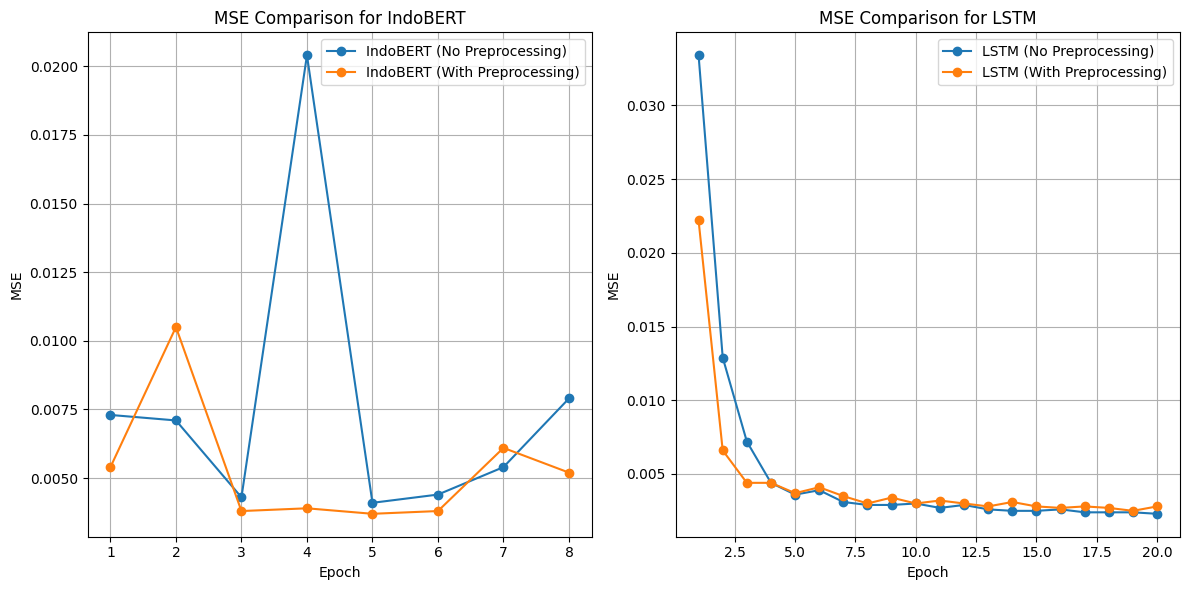
\includegraphics[width=0.95\textwidth]{images/mse comparison.png}
        \caption{Perbandingan Nilai \textit{Mean Squared Error} (MSE) antara Model IndoBERT dan LSTM pada Kondisi Dengan dan Tanpa \textit{Preprocessing}}
        \label{fig:grafik_training}
    \end{figure}
    
    Grafik tersebut menggambarkan perbandingan nilai Mean Squared Error (MSE) untuk dua model, yaitu IndoBERT dan LSTM, dalam dua kondisi, yaitu tanpa \textit{preprocessing} dan dengan \textit{preprocessing}.
   
    Pada grafik IndoBERT, terlihat adanya fluktuasi yang cukup signifikan pada kondisi tanpa \textit{preprocessing}, terutama di epoch ke-5, di mana nilai MSE mencapai puncak tertinggi sekitar 0.0200. Hal ini menunjukkan bahwa model mengalami kesulitan dalam mempelajari pola data dengan stabil. Sebaliknya, pada kondisi dengan \textit{preprocessing}, nilai MSE menunjukkan penurunan yang lebih konsisten dari awal hingga akhir, mengindikasikan bahwa \textit{preprocessing} membantu model dalam memahami data dengan lebih baik dan mempercepat proses konvergensi.

    Pada model LSTM, baik dengan maupun tanpa \textit{preprocessing}, nilai MSE terus menurun secara bertahap dari epoch awal hingga epoch terakhir. Meskipun terdapat sedikit perbedaan pada nilai awal MSE, kedua kondisi ini menunjukkan pola penurunan yang stabil dan mencapai nilai MSE yang relatif rendah pada akhir pelatihan. Hal ini menunjukkan bahwa model LSTM mampu mempelajari data secara efektif dalam kedua kondisi, meskipun \textit{preprocessing} tetap memberikan sedikit keunggulan dengan nilai MSE yang lebih rendah secara keseluruhan.

    \textit{Preprocessing} memberikan dampak positif bagi kedua model, terutama dalam mempercepat penurunan MSE dan meningkatkan stabilitas pelatihan. Model LSTM menunjukkan kemampuan yang lebih konsisten dalam mempelajari data, sementara model IndoBERT mengalami fluktuasi pada kondisi tanpa \textit{preprocessing}. \textit{Preprocessing} terbukti penting dalam membantu kedua model mencapai performa optimal.

    \item \textbf{Perbandingan Nilai MSE, MAE dan RMSE}
    \begin{figure}[H]
        \centering
        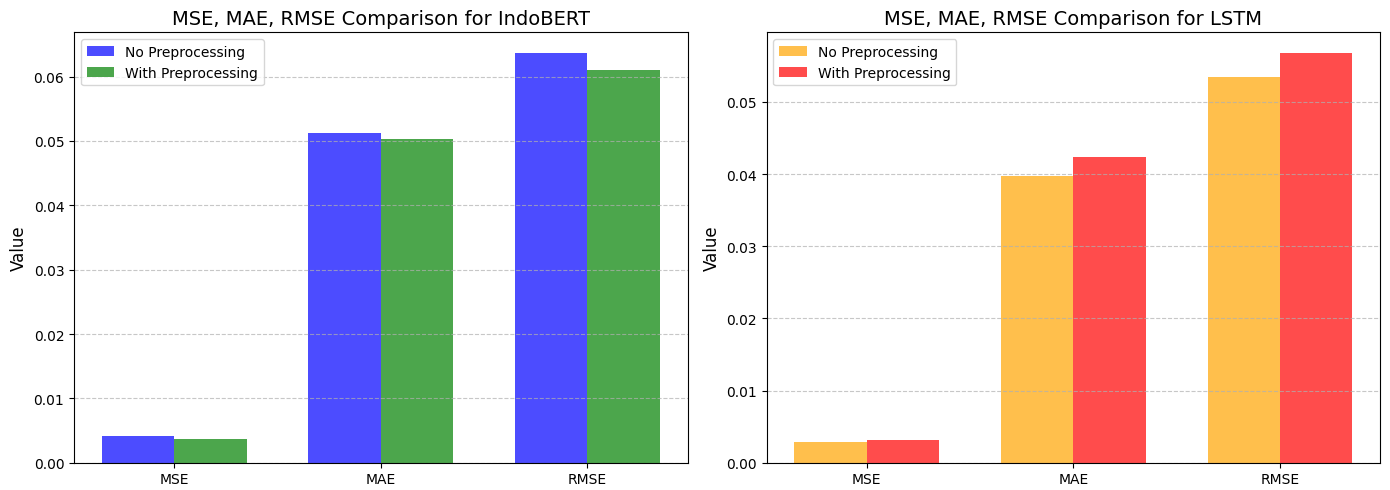
\includegraphics[width=0.95\textwidth]{images/mse, mae, rmse comparison.png}
        \caption{Perbandingan Nilai \textit{Mean Squared Error} (MSE), \textit{Mean Absolute Error} (MAE), dan \textit{Root Mean Squared Error} (RMSE) antara Model IndoBERT dan LSTM pada Kondisi Dengan dan Tanpa \textit{Preprocessing}}
        \label{fig:Perbandingan Nilai MSE, MAE dan RMSE}
    \end{figure}
    Grafik tersebut menggambarkan perbandingan \textit{Mean Squared Error} (MSE), \textit{Mean Absolute Error} (MAE), dan \textit{Root Mean Squared Error} (RMSE) antara model IndoBERT dan LSTM dengan dan tanpa \textit{preprocessing}.

    Model IndoBERT mengalami sedikit peningkatan performa setelah \textit{preprocessing} diterapkan. Nilai MSE menurun dari 0.0041 menjadi 0.0037, nilai MAE dari 0.0512 menjadi 0.0503, dan nilai RMSE dari 0.0637 menjadi 0.0610. Meskipun perubahan ini kecil, penurunan nilai-nilai kesalahan ini menunjukkan bahwa \textit{preprocessing} memberikan kontribusi positif terhadap akurasi model. Kesalahan yang berada di kisaran nilai tersebut menunjukkan bahwa rata-rata prediksi model sangat mendekati nilai sebenarnya, sehingga IndoBERT mampu menangani tugas ini dengan cukup akurat bahkan pada data yang kompleks seperti teks agama.

    Sebaliknya, model LSTM menunjukkan penurunan performa setelah \textit{preprocessing} diterapkan. Nilai MSE meningkat dari 0.0029 menjadi 0.0032, nilai MAE dari 0.0398 menjadi 0.0424, dan nilai RMSE dari 0.0535 menjadi 0.0568. Meskipun nilai-nilai ini masih relatif rendah, peningkatan kesalahan setelah \textit{preprocessing} menunjukkan bahwa \textit{preprocessing} tidak memberikan manfaat yang diharapkan pada LSTM. Hal ini mengindikasikan bahwa LSTM mungkin lebih peka terhadap perubahan data dan bisa bekerja lebih baik dengan data mentah.
    
    Secara keseluruhan, hasil ini menegaskan bahwa model IndoBERT mendapatkan manfaat dari \textit{preprocessing} dan dapat memberikan hasil yang konsisten, terutama ketika akurasi tinggi dibutuhkan. Di sisi lain, LSTM lebih cocok digunakan tanpa preprocessing dalam konteks ini, mengingat performanya yang lebih baik dengan data mentah. Nilai kesalahan yang rendah pada kedua model menunjukkan bahwa baik IndoBERT maupun LSTM mampu menangani tugas pengukuran keselarasan fatwa dengan Al-Quran dan Hadits dengan tingkat akurasi yang cukup baik, meskipun perbedaan kepekaan terhadap \textit{preprocessing} tetap menjadi faktor penting dalam pemilihan model.
    
    \item \textbf{Perbandingan Nilai \textit{R-Squared} (R²)}
    \begin{figure}[H]
        \centering
        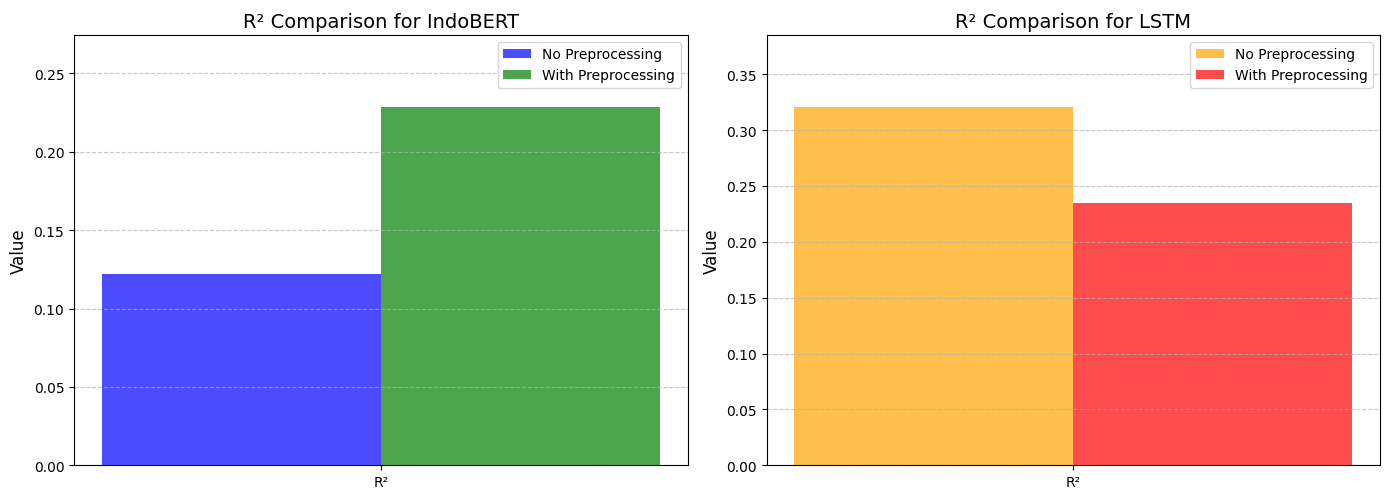
\includegraphics[width=0.95\textwidth]{images/r2 comparison.png}
        \caption{Perbandingan Nilai \textit{R-Squared} (R²) antara Model IndoBERT dan LSTM pada Kondisi Dengan dan Tanpa \textit{Preprocessing}}
        \label{fig:Perbandingan Nilai R-Squared}
    \end{figure}
    Grafik tersebut menggambarkan perbandingan koefisien determinasi R² antara model IndoBERT dan LSTM dengan dan tanpa \textit{preprocessing}. Koefisien determinasi R² mengukur seberapa baik model dapat menjelaskan variabilitas dalam data, dengan nilai yang lebih tinggi menunjukkan performa yang lebih baik.

   Pada model IndoBERT, terlihat peningkatan yang signifikan dalam nilai $R^2$ ketika \textit{preprocessing} diterapkan. Tanpa \textit{preprocessing}, nilai $R^2$ berada di sekitar 0,10, namun dengan \textit{preprocessing}, nilai ini meningkat hingga 0,25. Hal ini menunjukkan bahwa \textit{preprocessing} membantu IndoBERT lebih baik dalam menangkap pola dan hubungan dalam data, meningkatkan kemampuannya untuk menjelaskan variabilitas teks yang kompleks. Dengan kata lain, setelah \textit{preprocessing}, model IndoBERT mampu menjelaskan 25\% dari variabilitas dalam data, yang merupakan peningkatan signifikan dari 10\% sebelumnya.

    Sebaliknya, pada model LSTM, nilai $R^2$ justru mengalami penurunan ketika \textit{preprocessing} diterapkan. Tanpa \textit{preprocessing}, model menunjukkan nilai $R^2$ sekitar 0,33, namun setelah \textit{preprocessing}, nilai ini turun menjadi 0,23. Penurunan ini menunjukkan bahwa \textit{preprocessing} yang dilakukan mungkin menghilangkan informasi penting dari data atau membuat model kurang efektif dalam memahami pola. Meskipun nilai $R^2$ pada LSTM tanpa \textit{preprocessing} menunjukkan kemampuan model untuk menjelaskan 33\% dari variabilitas dalam data, penurunan ini menandakan bahwa \textit{preprocessing} tidak memberikan manfaat pada model ini dan malah mengurangi kemampuan LSTM dalam menangkap pola yang ada.
    
    Hasil ini menegaskan bahwa \textit{preprocessing} memiliki dampak yang berbeda pada kedua model. IndoBERT tampaknya mendapat manfaat signifikan dari \textit{preprocessing}, meningkatkan kemampuannya dalam memahami teks panjang dan kompleks. Dengan demikian, IndoBERT menjadi pilihan yang kuat jika \textit{preprocessing} merupakan bagian dari pipeline pengolahan data. Namun, hasil untuk LSTM mengindikasikan bahwa pendekatan \textit{preprocessing} yang digunakan perlu dievaluasi ulang. Kemungkinan besar, model ini lebih efektif dengan data mentah, atau mungkin memerlukan pendekatan \textit{preprocessing} yang lebih ringan dan sesuai. Hal ini penting karena LSTM sering kali lebih sensitif terhadap kehilangan informasi selama \textit{preprocessing}.
    
    Meskipun nilai $R^2$ pada kedua model menunjukkan hasil yang berbeda, nilai MSE, RMSE, dan MAE pada kedua model menunjukkan kinerja yang baik, dengan kesalahan yang relatif rendah. Metrik MSE, RMSE, dan MAE mengukur kesalahan prediksi model secara langsung, dan nilai yang lebih kecil menunjukkan bahwa model lebih akurat dalam memprediksi hasil yang mendekati nilai yang sebenarnya. Namun, nilai $R^2$ yang lebih rendah pada kedua model menunjukkan bahwa meskipun model dapat memberikan prediksi yang akurat secara numerik, model mungkin tidak sepenuhnya dapat menjelaskan pola yang mendasari hubungan antar data. Hal ini menunjukkan bahwa meskipun kesalahan numerik relatif kecil, model belum dapat menangkap keseluruhan variabilitas dalam data yang kompleks, yang tercermin dalam nilai $R^2$ yang rendah.
\end{itemize}

\subsection{Penentuan Treshold Keselarasan Fatwa}
Penentuan \textit{treshold} keselarasan dalam konteks mengukur keselarasan fatwa dengan Al-Quran dan Hadist merupakan langkah penting untuk memvalidasi apakah suatu fatwa memiliki kesesuaian atau relevansi yang cukup dengan sumber ajaran Islam. Salah satu cara untuk melakukan ini adalah dengan mengambil sampel pasangan teks fatwa dengan Al-Quran dan fatwa dengan Hadits pada masing-masing skor keselarasan 0.6, 0.7, dan 0.8 pada data \textit{training}, yang kemudian divalidasi oleh seorang ahli di bidang tersebut.

Berikut ini adalah penjelasan untuk masing-masing skor keselarasan yang diperoleh:

\begin{itemize}
    \item \textbf{Similarity 0.6} \\ \\
        \textbf{Fatwa}: \\
        1. Zakat fitrah hukumnya wajib dikeluarkan oleh setiap muslim atas dirinya dan jiwa yang menjadi tanggungannya saat menjelang Idul Fitri dengan ketentuan bahwa ia masih hidup pada malam hari raya dan memiliki kelebihan dari kebutuhan pokoknya untuk sehari. \\
        2. Zakat fitrah dibayarkan dalam bentuk makanan pokok. \\
        3. Kadar zakat fitrah adalah 1 sha' yang jika dikonversi ke beras menjadi 2,7 kg atau 3,5 liter. \\
        4. Zakat fitrah dapat dibayarkan dengan uang yang diamanahkan kepada panitia untuk dibelikan makanan pokok. \\
        5. Nilai zakat fitrah berupa beras, jika dinominalkan mengacu kepada:
        \begin{enumerate}[label=\alph*)]
            \item Harga jenis beras yang dikonsumsi muzakki.
            \item Sesuai dengan harga pasar setempat.
        \end{enumerate}
        6. Khusus bagi warga umat Islam yang makanan pokoknya bukan beras, maka zakat fitrah yang dikeluarkan sesuai dengan makanan pokok setempat. \\
        7. Menyegerakan pembayaran zakat fitrah sejak awal Ramadan hukumnya boleh. \\
        8. Waktu wajib membayar zakat fitrah adalah sebelum dilaksanakannya shalat Idul Fitri. \\
        9. Menyalurkan zakat fitrah yang diwakilkan oleh muzakki kepada badan/lembaga amil zakat atau panitia zakat fitrah melewati tanggal 1 Syawal hukumnya tidak sah kecuali ada uzur syar'i. \\
        10. Zakat fitrah ditasarufkan kepada fakir miskin. \\

        \textbf{Hadist}:\\
        "Telah menceritakan kepada kami [Abdan] dia berkata, telah mengabarkan kepada kami [Abdullah] telah mengabarkan kepada kami [Yunus] dari [Az Zuhri] dan dengan riwayat yang sama, telah menceritakan pula kepada kami [Bisyir bin Muhammad] berkata, telah mengabarkan kepada kami [Abdullah] berkata, telah mengabarkan kepada kami [Yunus] dan [Ma'mar] dari [Az Zuhri] seperti lainnya berkata, telah mengabarkan kepada kami [Ubaidullah bin Abdullah] dari [Ibnu 'Abbas] berkata, bahwa Rasulullah shallallahu 'alaihi wasallam adalah manusia yang paling lembut terutama pada bulan Ramadlan ketika malaikat Jibril 'Alaihis Salam menemuinya, dan adalah Jibril 'Alaihis Salam mendatanginya setiap malam di bulan Ramadlan, dimana Jibril 'Alaihis Salam mengajarkan Al Qur'an. Sungguh Rasulullah shallallahu 'alaihi wasallam jauh lebih lembut daripada angin yang berhembus." \\

        \textbf{Analisis}:\\
        Pada skor similarity 0.6, terdapat keselarasan antara Fatwa dan Hadits yang cukup, namun tidak sepenuhnya mendalam. Fatwa mengenai zakat fitrah menjelaskan beberapa ketentuan penting terkait kewajiban zakat fitrah, seperti waktu pembayaran, syarat, dan bagaimana zakat fitrah dihitung dan didistribusikan.

        Namun, Hadits yang disertakan dalam teks ini lebih berbicara tentang kelembutan Rasulullah dan interaksi beliau dengan malaikat Jibril di bulan Ramadan, tanpa mengarah secara langsung pada perincian zakat fitrah. Meskipun ada hubungan dalam konteks ibadah Ramadan (di mana zakat fitrah dikeluarkan pada akhir Ramadan), Hadits ini tidak secara eksplisit menjelaskan ketentuan zakat fitrah atau kewajibannya. Hadits ini lebih banyak menggambarkan kelembutan Rasulullah selama bulan Ramadan.

    \item \textbf{Similarity 0.7} \\\\
        \textbf{Fatwa}: \\
        1. Melihat mushaf al-Qur'an saat shalat tidak membatalkan shalat.\\
        2. Membaca ayat Al-Qur'an dengan cara melihat mushaf bagi orang yang sedang shalat hukumnya diperbolehkan jika ada kebutuhan, sepanjang tidak mengganggu kekhusyu'an dan tidak dilakukan dengan gerakan yang membatalkan shalat.\\
        3. Untuk menjaga kekhusyu'an dalam shalat, imam shalat diutamakan untuk membaca ayat al-Qur'an dengan hafalan (bil ghaib), tanpa melihat mushaf.\\

        \textbf{Hadist}: \\
        "Dan telah menceritakan kepadaku [Nashr bin Ali Al Juhdlami] telah menceritakan kepada kami [Bisyr yaitu Ibn Al Mufadlal] dari [Khalid] dari [Anas bin Sirin] katanya; aku mendengar [Jundab bin Abdullah] berkata; Rasulullah shallallahu \'alaihi wasallam bersabda: "Barangsiapa shalat subuh, maka ia berada dalam jaminan Allah, oleh karena itu jangan sampai Allah menuntut sesuatu dari kalian sebagai imbalan jaminan-Nya, sehingga Allah menangkapnya dan menyungkurkannya ke dalam neraka jahannam." \\

        \textbf{Analisis}: \\
        Pada skor \textit{similarity} 0.7, terdapat keselarasan yang cukup antara Fatwa dan Hadits, meskipun keduanya membahas aspek yang berbeda dari shalat. Fatwa lebih fokus pada praktik teknis shalat, terutama mengenai melihat mushaf al-Qur'an selama shalat, yang diperbolehkan jika tidak mengganggu kekhusyu'an. Fatwa ini juga menekankan pentingnya imam untuk membaca ayat Al-Qur'an dengan hafalan untuk menjaga kekhusyu'an dalam shalat. 
        
        Sementara itu, Hadits yang disertakan lebih berbicara tentang keutamaan shalat subuh dan jaminan Allah bagi mereka yang melaksanakan shalat tersebut dengan benar, serta ancaman bagi yang tidak menjaga amanah shalat mereka. Keduanya tetap terkait dengan pentingnya menjaga kualitas shalat, baik dalam hal kekhusyu'an maupun dalam pelaksanaannya yang benar. Namun, meskipun ada keselarasan dalam topik besar mengenai shalat, perbedaan dalam konteks pembahasannya menunjukkan bahwa hubungan keduanya tidak sepenuhnya mendalam.

    \item \textbf{Similarity 0.8} \\\\
        \textbf{Fatwa}: \\
        Makan daging babi diharamkan dalam Islam berdasarkan dalil-dalil dari Al-Qur'an dan Hadis. Dalam Al-Qur'an, Allah berfirman: 'Sesungguhnya Allah hanya mengharamkan bagimu bangkai, darah, daging babi, dan apa yang disembelih dengan menyebut nama selain Allah...' (QS. Al-Baqarah: 173).\\

        \textbf{Al-Quran}: \\
        'Sesungguhnya Allah hanya mengharamkan atasmu bangkai, darah, daging babi, dan (hewan) yang disembelih dengan (menyebut nama) selain Allah. Akan tetapi, siapa yang terpaksa (memakannya) bukan karena menginginkan dan tidak (pula) melampaui batas, sesungguhnya Allah Maha Pengampun lagi Maha Penyayang.'\\

        \textbf{Analisis}: \\
        Pada skor similarity 0.8, terdapat keselarasan yang sangat erat antara Fatwa dan Al-Qur'an terkait keharaman daging babi dalam Islam. Fatwa secara eksplisit merujuk pada dalil dari Al-Qur'an yang melarang konsumsi daging babi, seperti yang disebutkan dalam QS. Al-Baqarah ayat 173. Ayat ini menjelaskan bahwa Allah mengharamkan bangkai, darah, daging babi, serta hewan yang disembelih dengan menyebut nama selain Allah, kecuali dalam kondisi darurat di mana konsumsi diizinkan tanpa melampaui batas.

        Keselarasan ini terlihat jelas karena Fatwa menyampaikan esensi yang sama dengan ayat Al-Qur'an, yaitu larangan konsumsi daging babi yang bersifat tegas, namun dengan pengecualian dalam keadaan terpaksa. Oleh karena itu, skor similarity 0.8 dapat dianggap tepat karena hubungan antara Fatwa dan ayat Al-Qur'an sudah sangat kuat, baik dalam konteks isi maupun makna, sehingga tidak memerlukan interpretasi tambahan.
\end{itemize}

Nilai \textit{similarity} 0.8 dipilih sebagai \textit{threshold} keselarasan karena pada level ini, fatwa dan Hadist sudah menunjukkan hubungan yang sangat erat dan relevansi yang kuat. Pada nilai ini, model sudah cukup mampu mengidentifikasi dan memetakan hubungan antara teks fatwa dengan sumber dari Al-Quran dan Hadist. Oleh karena itu, \textit{threshold} 0.8 ditetapkan sebagai batas yang optimal, karena pada level ini, keselarasan antara fatwa dan Hadits dapat dianggap sangat konsisten dan mendalam, sehingga cocok untuk dijadikan rujukan atau penerimaan tanpa perlu banyak interpretasi lebih lanjut.

% 5. Conclusion
\section{Kesimpulan}
Hasil penelitian menunjukkan bahwa AI dapat memberikan kontribusi signifikan dalam penafsiran hukum agama dan mendukung lembaga agama dalam mengeluarkan fatwa yang sesuai dengan ajaran-ajaran yang terkandung dalam sumber-sumber agama tersebut. Berdasarkan hasil pengujian model, meskipun nilai $R^2$ pada kedua model yang digunakan menunjukkan skor yang relatif rendah, metrik MSE, RMSE, dan MAE menunjukkan kinerja yang baik dengan kesalahan yang relatif rendah. Pemilihan \textit{threshold similarity} 0.8 terbukti optimal karena pada level ini, fatwa dan hadist sudah menunjukkan hubungan yang sangat erat, dengan keselarasan yang konsisten dan relevan, yang cukup untuk dijadikan rujukan atau penerimaan tanpa perlu banyak interpretasi lebih lanjut.

Ke depan, untuk meningkatkan hasil yang lebih akurat, disarankan untuk mencoba menggunakan model deep learning lain yang lebih kompleks, guna memperoleh nilai $R^2$ yang lebih tinggi. Selain itu, pengembangan model \textit{clustering} teks berdasarkan topik juga disarankan untuk mengelompokkan teks berdasarkan tema atau kategori tertentu. Pendekatan ini diharapkan dapat memperkaya analisis dan memberikan wawasan yang lebih dalam mengenai keselarasan antara fatwa dan hadist, serta membantu dalam pengambilan keputusan yang lebih tepat dalam konteks hukum agama.


\newpage
\bibliographystyle{plain}
% Add your bibliography entries here

\begin{thebibliography}{9}

\bibitem{Jamaa2018} Jamaa, L. (2018). Fatwas of the Indonesian council of ulama and its contributions to the development of contemporary Islamic law in Indonesia. *Indonesian Journal of Islam and Muslim Societies, 8*(1), 29–56. https://doi.org/10.18326/ijims.v8i1.29-56
\bibitem{Juarto2023} Juarto, B. (n.d.). Indonesian news classification using IndoBert. *International Journal of Intelligent Systems and Applications in Engineering, 11*(2), 454–460. www.ijisae.org
\bibitem{Hakim2023} Hakim, L., and Azizi, M. R. (2023). Otoritas Fatwa Keagamaan dalam Konteks Era Kecerdasan Buatan (Artificial Intelligence/AI). Jurnal Ilmiah Ar-Risalah: Media Ke-Islaman, Pendidikan dan Hukum Islam, 21(2), 164-174.
\bibitem{Zayed2015} Zayed, R. A., Hady, M. F. A., and Hefny, H. (2015, April). Islamic fatwa request routing via hierarchical multi-label Arabic text categorization. In 2015 First International Conference on Arabic Computational Linguistics (ACLing) (pp. 145-151). IEEE.
\bibitem{Rohman2023} Rohman, F., Azizah, H. A., Ardianti, D., and Noor, A. M. (2023). ISLAM IN THE MIDDLE OF AI (Artificial Intelligence) STRUGGLE: BETWEEN OPPORTUNITIES AND THREATS. At-Tuhfah, 12(1), 19-27.
\bibitem{Alhawarat2015} Alhawarat, M., Hegazi, M., and Hilal, A. (2015). Processing the text of the Holy Quran: a text mining study. International Journal of Advanced Computer Science and Applications, 6(2), 262-267.
\bibitem{Kuligowska} K. Kuligowska and B. Kowalczuk, "Pseudo-labeling with transformers for improving Question Answering systems," Procedia Computer Science, vol. 192, pp. 1162-1169, 2021. doi: 10.1016/j.procs.2021.08.119.
\bibitem{J.Han} J. Han, M. Kamber, and J. Pei, "2 - Getting to Know Your Data," in Data Mining, 3rd ed., The Morgan Kaufmann Series in Data Management Systems, J. Han, M. Kamber, and J. Pei, Eds. Morgan Kaufmann, 2012, pp. 39-82. doi: 10.1016/B978-0-12-381479-1.00002-2.
\bibitem{hochreiter1997long} S. Hochreiter and J. Schmidhuber, "Long short-term memory," Neural Computation, vol. 9, no. 8, pp. 1735-1780, 1997. doi: 10.1162/neco.1997.9.8.1735.
\bibitem{Graves} A. Graves, "Generating Sequences With Recurrent Neural Networks," arXiv, 2013. doi: 10.48550/arXiv.1308.0850.
\bibitem{Kingma} D. P. Kingma and J. Ba, "Adam: A Method for Stochastic Optimization," arXiv, 2014. doi: 10.48550/arXiv.1412.6980.
\bibitem{mse} Z. Zhao, L. Alzubaidi, J. Zhang, Y. Duan, and Y. Gu, "A comparison review of transfer learning and self-supervised learning: Definitions, applications, advantages and limitations," Expert Systems with Applications, vol. 242, p. 122807, 2024. doi: 10.1016/j.eswa.2023.122807.
\bibitem{rmse} S. K. Jain and V. P. Singh, "Chapter 4 - Statistical Techniques for Data Analysis," in Developments in Water Science, vol. 51, S. K. Jain and V. P. Singh, Eds. Elsevier, 2003, pp. 207-276. doi: 10.1016/S0167-5648(03)80058-8.
\bibitem{mae} G. Xia, Y. Bi, and C. Wang, "Optimization design of passive residual heat removal system based on improved genetic algorithm," Annals of Nuclear Energy, vol. 189, p. 109859, 2023. doi: 10.1016/j.anucene.2023.109859.
\bibitem{r2}G. Romeo, "Chapter 13 - Data analysis for business and economics," in Elements of Numerical Mathematical Economics with Excel, G. Romeo, Ed. Academic Press, 2020, pp. 695-761. doi: 10.1016/B978-0-12-817648-1.00013-X.
\end{thebibliography}


\end{document}